\section{Cloud Architecture and Design}

This system will be deployed using Infrastructure as a Service (IaaS) on Amazon Web Services (AWS).

\subsection{Cloud Provider Selection}
The growth in popularity of cloud services has fostered an industry with many competing cloud providers. Given the continued growth of the SmartV user-base, the choice to leverage an existing provider has been made to balance the increasing but dynamic demands of the platform while maintaining minimal-cost cloud infrastructure. Both internal and public cloud providers have been considered, including offerings from VMware, OpenStack, Azure, AWS.

The use of internal cloud provisioning necessitates a significant up-front cost in both the hardware and software required by the transition to cloud infrastructure, and is over-all less flexible than the infrastructure-as-a-service models provided by Azure and AWS. These caveats to an internal cloud deployment represent unnecessary additional costs and management responsibilities to SmartV, reducing the organisations focus on end-users.

For these reasons and over-all compatibility with the business requirements outlined in section \ref{sec:businessrequirements} AWS is selected as the cloud provider of choice for the project. The use of AWS also allows SmartV to bypass the upfront cost of any immediate upgrades to physical infrastructure by instead utilising storage, compute, and network provided by the AWS platform, paying for only the resources used by SmartV. The choice of AWS is also influenced by the ready availability of high-power compute instances required by the SmartV platform (see section \ref{sec:infrastructure-components}).

\subsection{Design Assumptions}\label{sec:designassumptions}

The preparation of this document makes a few key assumptions that will need to be confirmed with SmartV. These are the following: 

\begin{enumerate}
    \item \textbf{Provision of Software:} It is assumed that SmartV has proprietary software suitable for serving the needs of its customer base, and is only looking to extend from an on-premises computing solution to a cloud infrastructure solution. No consideration is made for changes to software not directly related to infrastructure.
    \item \textbf{Geographic Scope:} It is assumed that SmartV operates primarily in the Asia-Pacific (APAC) region. We therefore design for traffic in the area by placing infrastructure primarily in Sydney datacentres, with high availability available in Singapore datacentres.
    \item \textbf{User Accounts:} It is assumed that SmartV has interest in individual user profiles and accounts, which will need special consideration in this infrastructure environment to handle storage and backups.
    \item \textbf{Compute Requirements:} It is assumed that the SmartV software requires high levels of compute power to provide multi-media services to users. Therefore we spec the compute capabilities quite highly, with support for high CPU, GPU, and RAM availability per instance.
\end{enumerate}

\subsection{Infrastructure Design}

The architecture of the cloud infrastructure has been designed to reflect the business requirements listed in section \ref{sec:businessrequirements} and the design assumptions provided in section \ref{sec:designassumptions}. A brief overview of the deployed infrastructure is provided here, with details of each component provided in section \ref{sec:infrastructure-components} and a summary of implemented features in \textbf{PUT REFERENCE HERE}.

All public-facing infrastructure components are routed from users to the AWS cloud via AWS's managed DNS service Route 53 connected directly to an application load balancer (ALB). The ALB allows automatic allocation of users amongst the distributed systems responsible for providing the SmartV services, and can automatically redistribute users to working infrastructure in the case of partial system failures. The ALB is provisioned within a public subnet in a Virtual Private Cloud (VPC), allowing end users to directly access only the ALB and not the internal infrastructure it directs traffic to.

SmartV services themselves will be hosted on AWS Elastic Compute Cloud (EC2) instances provisioned across multiple availability zones (AZs) within internal subnets in the VPC. The distribution of instances across AZs provides a high level of redundancy and fault tolerance. In the event of hardware failures or other disruptions in one availability zone, SmartV's services will remain operational, offering uninterrupted access to users. The placement of the EC2 instances within an internal subnet restricts direct connectivity to the SmartV hosts, reducing the risk of unauthorised access and enhancing overall security. This configuration ensures that SmartV hosts are shielded from direct exposure to the internet, providing an additional layer of protection for sensitive data and services.

The EC2 instances are also configured as part of an auto scaling group, allowing the number of provisioned instances to fluctuate with demand and provide end users with consistent performance independent of overall service load. The use of an ALB allows this scaling to be performed without any service interruptions, as traffic will be automatically routed to the most appropriate EC2 instance.


All unstructured blob data (i.e. user multi-media files) is hosted on AWS Simple Storage Service (S3), with structured user data (login details, preferences) held in AWS Relational Database Service (RDS). Both S3 and RDS are configured with data encryption and backups, ensuring secure and reliable data storage and transfer \parencite{amazonwebservicesEncryptingAmazonRDS2023, amazonwebservicesProtectingDataEncryption}.

An architecture diagram of the SmartV cloud infrastructure is provided in figure \ref{fig:awsdiagram}.

\begin{figure}[h]
    \centering
    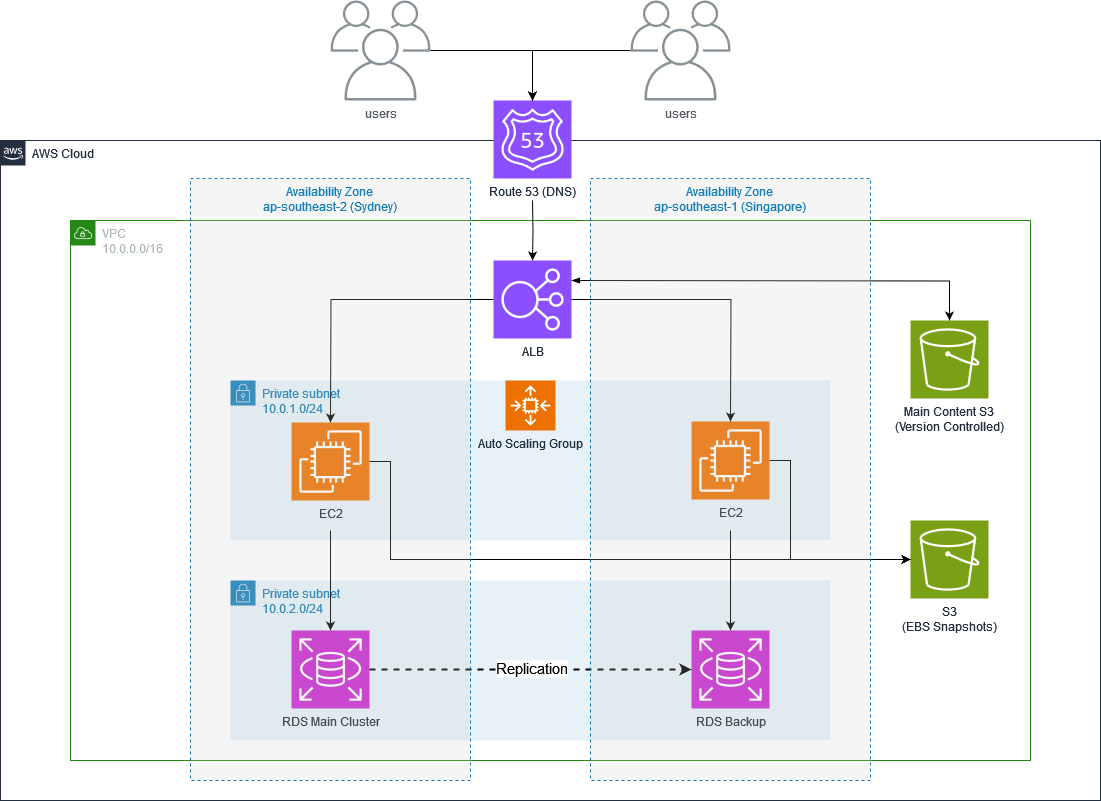
\includegraphics[width=\textwidth]{cci_aws}
    \caption{Cloud Infrastructure Topology}
    \label{fig:awsdiagram}
\end{figure}


\subsection{Infrastructure Components}
\label{sec:infrastructure-components}

\subsubsection*{DNS (Route 53)}

Allowing global access through http, a DNS record is needed and will be achieved through an AWS Route 53 domain. This will transfer users to the ALB.

\subsubsection*{Network (ALB)}

To balance load across seperate compute clusters, an application load balancer (ALB) will handle distribution of incoming requests to allow transparent scaling of compute abstracted from the user, meaning bucekts of storage can scale infinitely.

\subsubsection*{Compute (EC2)}

Using an autoscaling group of EC2 instances of type ``p3.8xlarge'', compute will be handled and scaled with demand. The instance types are very large to accomodate for the intense RAM, CPU, and GPU requirements video demands. A key feature of S3 is the inherent scalability, as this is abstracted away from the end user. The use of this instance scale also allows networking performance of 10 Gbps. This will be very helpful as the most intense network requirements are occurring internally on AWS, between compute and content storage on S3.

\subsubsection*{Content Storage (S3)}

AWS Simple Storage Service (S3) allows for cheap and easy object storage through a HTTP API endpoint. This is suitable for storing the large files used by the service, and allowing avilability across the platform.

\subsubsection*{Backup Storage (S3)}

Snapshots of the drives associated with compute instances, the elastic block storage (EBS) drives, will be palced daily in a seperate S3 bucket to allow disaster recovery of user's work and files retained locally on the compute instance.

\subsubsection*{User Database (RDS)}

AWS Relational Database System (RDS) will be used to handle user information such as login, account details, and payment information. Using a traditional database system is suitable over S3 as it allows structure and replication.

\subsubsection*{Network (Public)}

The entire cloud system will exist within a private VPC, with the only publically exposed element being the ALB accessible through the Route 53 DNS record or associated IP address.

\subsubsection*{Network (Internal)}

Internally, the platform is networked through a private IPv4 subnet in CIDR block 10.0.0.0/16. Each private subnet in turn has it's own CIDR block with a netmask of 24. Compute and the RDS service reside in seperate private subnets to improve security.

\subsection{Pricing}

Utilising scalable infrastructure as a service makes accurate, fixed estimations of costs difficult as prices are tied directly to utilisation. Here an estimate of month-to-month costs is provided as calculated via the AWS pricing calculator\footnote{See \url{https://calculator.aws}.}

% https://calculator.aws/#/addService
